\section{Disjoint domains, cone chains, and an integral detector}
\label{sec:domains}

The fixed-contact polygon bound will supply both disjoint analytic domains
and the integral detector.  We first show that every finite family can be
peeled: one sheet
meets the remaining sheets only inside a vertex set whose incident edges
form a forest.  Peeling gives a unique decomposition of every finite Cayley
cycle into sheet cycles.  From these cycle coordinates the argument
branches.  A compactness argument produces disjoint domains and a residual
forest for the analytic realization.  Independently, coning the full sheets
gives an exact cellular complex, which proves torsion-freeness and extends
an integral detector from the Heisenberg torus to the ambient group.

Write $\mathcal C$ for the formal right Cayley graph of $\Gamma$ supplied by
Proposition~\ref{prop:graphical-realization}.  A positive edge is a separate
cell $(g,\sigma)$, directed from $g$ to $g\sigma$; cells with the same unordered
endpoints are not identified.  Let $\mathcal Q$ be the family of distinct
translated images of the connected cover $\widetilde X$.  Each $Q\in\mathcal Q$
retains its intrinsic graph metric and the type of each of its vertices in
$X$.  In particular, ``old'' and ``private'' refer to the vertex in that
sheet, not just to its physical image in $\mathcal C$.

We use the following conclusions of
Lemma~\ref{lem:private-completion},
Proposition~\ref{prop:graphical-realization}, and
Lemma~\ref{lem:sheet-polygon}.  The sheets are embedded, their stabilizers
are conjugates of $\HH$, and every private vertex has only private incident
edges.  Enlarging the fixed degree constant absorbs the six added
incidences, so the maximum intrinsic degree is at most
$\Delta\leq K_{b,\epsilon}D$.  On each sheet the scale function $m_Q$ satisfies
\begin{equation}
 \abs{m_Q(u)-m_Q(v)}\leq a\,d_Q(u,v),\qquad
 a=\frac{b}{\log_2q}\leq10^{-6},\qquad m_Q\geq10^6.
 \label{eq:domain-scale}
\end{equation}
At an old vertex in layer $i$, its value is $m_i=H_i/\log_2q$.
Every simple circuit in $Q$, based at $v$, has length greater than
$6.03m_Q(v)$.  Here a comparison arc is an arc in the reduced
fixed-contact filling of Lemma~\ref{lem:sheet-polygon}.  Every such arc
has length less than
$L m_Q(v)$ when read from either endpoint $v$, where $L=1.003$, and contains
no private edge.  Finally, a polygon through $k\geq2$ distinct sheets,
with its contact vertices fixed, has a reduced filling whose exterior
boundary has at most $4k-6$ comparison-arc incidences, counting both
traversals of an exterior bridge.  Each entire nonconstant side is a
concatenation of those arcs.  The last fixed-endpoint assertion will be
used even when a contact vertex is private.

\subsection{Finite peeling, including private contacts}

Put $\kappa=3.014$.  If a path is a concatenation of at most three comparison
arcs and starts at $v$, the successive initial scales are at most
$m_Q(v)$, $(1+La)m_Q(v)$, and $(1+La)^2m_Q(v)$.  Consequently its length
is less than
\begin{equation}
 L\bigl(1+(1+La)+(1+La)^2\bigr)m_Q(v)
 <3.010m_Q(v)<\kappa m_Q(v).
 \label{eq:three-domain-arcs}
\end{equation}
Indeed the coefficient on the left is
$3.009+3.018027a+1.009027027a^2$, which is less than $3.010$ for
$a\leq10^{-6}$.

For a vertex set $B\subseteq V(Q)$, let $\operatorname{Star}_Q(B)$ denote
the subgraph consisting of all edges of $Q$ with at least one endpoint
in $B$, together with their endpoints.  This is an edge-incidence
neighborhood, rather than the induced graph on $B$.

\begin{lemma}[Allowed removed sets]
\label{lem:allowed-domain-sets}
For an old vertex $v\in Q$, set
\[
 B_Q(v)=\{w\in V(Q):d_Q(v,w)\leq\lfloor\kappa m_Q(v)\rfloor\}.
\]
The graphs $\operatorname{Star}_Q(B_Q(v))$ and
$\operatorname{Star}_Q(\{w\})$, for a private vertex $w$, are forests.
The empty set also has this property.

After increasing $s$ as permitted by the parameter order, if $B_Q(v)$
contains an old vertex of layer $i$, then
\begin{equation}
 \abs{B_Q(v)}\leq 2^{10H_i}.
 \label{eq:domain-ball-cardinality}
\end{equation}
A private singleton contains no old vertex.
\end{lemma}

\begin{proof}
Let $m=m_Q(v)$ and $R=\lfloor\kappa m\rfloor$.  All vertices of the
induced ball $B_Q(v)$ can be joined to $v$ by paths inside that ball;
choosing a predecessor at distance one less gives a shortest-path tree.
If the ball had a non-tree edge, that edge and its tree path would
contain a simple circuit of length at most $2R+1$.  If an outside vertex
had two edge incidences into the ball, these incidences and a path in
the tree would contain a simple circuit of length at most $2R+2$.
This includes the possibility of parallel edges.  Either circuit has
a vertex $u$ in the ball, at which
$m_Q(u)\geq m-aR\geq(1-\kappa a)m$.  Both possibilities contradict
the local girth bound, because
\begin{equation}
 6.03(1-\kappa a)m>2\kappa m+2\geq2R+2.
 \label{eq:domain-ball-girth}
\end{equation}
For the declared parameters, the difference between the first two
expressions is at least
$(0.002-6.03\kappa\cdot10^{-6})10^6-2>0$.
Thus the ball is a tree and each outside vertex has at most one edge
incidence into it.  Its incidence neighborhood is a tree with possible
additional leaves, hence a forest.  The incidence neighborhood of a
singleton is a star: loops or repeated neighbors would give a circuit
of length one or two, which the same local girth bound excludes.

The constants in $K_{b,\epsilon}$ are fixed before $s$.  Since
$\log_2D=.60005s$, we may arrange
$\log_2(\Delta+1)\leq .61s$.  The ball has at most
$(\Delta+1)^{R+1}$ vertices.  If an old vertex of layer $i$ lies in it,
Equation~\eqref{eq:domain-scale} gives
$m\leq m_i/(1-\kappa a)$.  Therefore
\[
 \log_2\abs{B_Q(v)}
 \leq\left(\frac{\kappa m_i}{1-\kappa a}+1\right).61s
 =H_i\left(
 \frac{.61\kappa}{.50005(1-\kappa a)}
 +\frac{.61}{.50005m_i}\right)<4H_i<10H_i.
\]
The displayed strict estimate follows from $a\leq10^{-6}$ and
$m_i\geq10^6$.  This proves Equation~\eqref{eq:domain-ball-cardinality}.
\end{proof}

For an allowed removed set $R_Q$, write $D_Q=V(Q)\setminus R_Q$.
Figure~\ref{fig:allowed-domains} illustrates the two nonempty choices
and their incidence neighborhoods.
\begin{figure}[tbp]
  \centering
  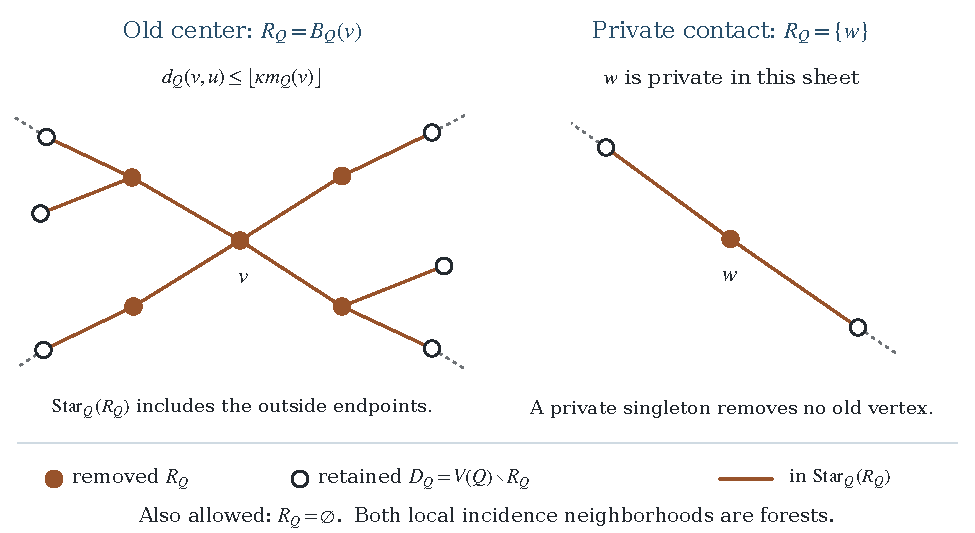
\includegraphics[width=\linewidth]{figures/allowed-domains.pdf}
  \caption{Schematic incidence neighborhoods of allowed removed sets:
  an old-centered ball or a private singleton of degree two. Filled
  vertices lie in $R_Q$; hollow vertices remain in $D_Q$.
  Colored edges have an endpoint in $R_Q$, so their outside endpoints
  also belong to $\operatorname{Star}_Q(R_Q)$. These neighborhoods are
  forests by Lemma~\ref{lem:allowed-domain-sets}. Dashed continuations
  represent unspecified sheet paths. Graph-metric lengths and
  cardinalities are not drawn to scale.}
  \label{fig:allowed-domains}
\end{figure}

For a finite family $\mathcal F\subseteq\mathcal Q$, the contact set of
$Q\in\mathcal F$ is
\[
 I_{\mathcal F}(Q)=V(Q)\cap
       \bigcup_{R\in\mathcal F\setminus\{Q\}}V(R).
\]
These sets need not be finite.  In particular, the fact that comparison
arcs have no private edges does not exclude a singleton contact at a
private vertex.  The next lemma includes that case explicitly.

\begin{lemma}[Finite peeling]
\label{lem:sheet-peeling}
Every nonempty finite family $\mathcal F$ has a sheet $Q$ for which
$I_{\mathcal F}(Q)$ is either empty, contained in $B_Q(v)$ for some old
contact $v$, or equal to a singleton private contact.
Consequently the family can be ordered $Q_1,\ldots,Q_n$ with allowed
removed sets $R_j$ of those three forms such that
\begin{equation}
 V(Q_j)\cap\bigcup_{\ell>j}V(Q_\ell)\subseteq R_j.
 \label{eq:finite-peeling-overlap}
\end{equation}
\end{lemma}

\begin{proof}
Suppose that no sheet has one of the three properties.  Every sheet
then has a contact.  We will construct a polygon in distinct sheets with
all but one side forced to use either a private edge or at least four
comparison arcs.  The exterior-arc bound will exclude this polygon.

Enter a sheet at a contact $u$.  If $u$ is old,
choose a contact $w\notin B_Q(u)$; its integer distance from $u$ is
strictly greater than $\kappa m_Q(u)$.  If $u$ is private, choose any
contact $w\ne u$, which is possible because the contact set is not
that private singleton.  Transfer at $w$ to another sheet containing
it and repeat.  Since the family is finite and consecutive sheets
are different, a sheet eventually repeats.  At the first repetition,
retain the intervening $k\geq2$ distinct sheets and close the path
inside the repeated sheet.  The resulting polygon has $k-1$ chosen
nonconstant sides; only the closing side is unrestricted.

Apply Lemma~\ref{lem:sheet-polygon} with all these contact vertices
fixed.  If a chosen side has a private endpoint in its sheet, any
nonconstant path with those endpoints starts or ends with a private
 edge.  Some private edge is therefore unavoidable in every replacement
 path with the same distinct endpoints.  Yet every arc of the reduced
side is a comparison arc, none of which contains a private edge.
This is impossible.  Otherwise all $k-1$ chosen sides have old
endpoints and have intrinsic endpoint distance greater than
$\kappa m_Q(u)$ at their incoming contacts.  By
Equation~\eqref{eq:three-domain-arcs}, each such side requires at least
four exterior arc incidences.  There are therefore at least
$4(k-1)>4k-6$ exterior incidences, again a contradiction.  The argument
does not require the closing side to be nonconstant or long.

Remove the sheet just obtained and apply the same assertion to the
remaining finite family.  At each removal take its whole contact ball,
its private singleton, or the empty set, respectively.  This gives
Equation~\eqref{eq:finite-peeling-overlap}.
\end{proof}

\subsection{Finite cycle coordinates}

An oriented edge chain over a commutative ring $R$ always means a
finite-support chain.  The cycle module of a graph $Y$ is
$Z_1(Y;R)=\ker(\partial:C_1(Y;R)\to C_0(Y;R))$.  A forest has no
nonzero such cycle: the support of a proposed cycle is a finite forest,
and its coefficient at an edge incident to a leaf must vanish; repeated
leaf removal removes the whole support.

\begin{lemma}[Direct cycle coordinates]
\label{lem:sheet-cycle-coordinates}
For every commutative coefficient ring $R$, the sum of the inclusions
is an isomorphism
\begin{equation}
 \Phi_R:\bigoplus_{Q\in\mathcal Q}Z_1(Q;R)
       \longrightarrow Z_1(\mathcal C;R),\qquad
       (c_Q)_Q\longmapsto\sum_Qc_Q.
 \label{eq:sheet-cycle-isomorphism}
\end{equation}
Both the direct sum and every chain appearing here have finite support.
\end{lemma}

\begin{proof}
First, every finite cycle chain in a graph is a finite linear
combination of circuit chains.  To see this, take a spanning forest
of its finite support graph.  For each edge outside that forest,
subtract its coefficient times the circuit formed with the forest
path between its endpoints.  This removes all edges outside the
forest.  The remainder is a cycle supported on a forest and is zero.
Loops and pairs of parallel edges are included in this argument.

Let a circuit in $\mathcal C$ start at $g$ and read the word $w$.
The definition of $\Gamma$ means that, in the free group on the
formal labels, $w$ is a finite product of conjugates of words read on
closed walks of $\widetilde X$, and their inverses.  Follow that
product from $g$ in $\mathcal C$.  Each conjugating stem is traversed
once in each direction, so its oriented chain cancels.  Each relator
walk lies in a translated sheet.  Free cancellation of adjacent
inverse letters also cancels the corresponding oriented edge chains
in the formal Cayley graph.  Thus the circuit chain is a finite sum
of sheet cycle chains.  The preceding circuit decomposition proves
surjectivity of $\Phi_R$.

For injectivity, suppose that $\sum_{j=1}^n c_{Q_j}=0$.  Order the
finitely many sheets in this relation by Lemma~\ref{lem:sheet-peeling}.
An edge of $Q_1$ with a nonzero coefficient in $c_{Q_1}$ must occur
in another nonzero coordinate, since the total coefficient is zero.
Both endpoints of that edge are contacts with a later sheet and
belong to $R_1$.  Hence $c_{Q_1}$ is supported on
$\operatorname{Star}_{Q_1}(R_1)$, a forest by
Lemma~\ref{lem:allowed-domain-sets}, and is zero.  Remove this
coordinate and repeat.  Every coordinate is zero.
\end{proof}

\subsection{Simultaneous domains for the analytic realization}

We now choose removed sets on all sheets at once, so that the retained
domains are disjoint and every Cayley circuit contains an edge internal to
one of them.  The cycle coordinates just proved provide finite witnesses
for this second requirement, allowing both requirements to pass to a limit.

\begin{proposition}[Simultaneous disjoint domains]
\label{prop:domains}
There are sets $R_Q\subseteq V(Q)$, one for each sheet, such that each
$R_Q$ is empty, an old-centered ball $B_Q(v)$, or a private singleton,
and the sets $D_Q=V(Q)\setminus R_Q$ have the following properties.
\begin{enumerate}
 \item The physical vertex sets $D_Q$ are pairwise disjoint.
 \item Put
 \[
 E_{\mathrm{int}}=
 \bigcup_{Q\in\mathcal Q}
 \{e\in E(Q):\text{both endpoints of }e\text{ lie in }D_Q\}.
 \]
 Every edge in this union has a unique such sheet, and
 $(V(\mathcal C),E(\mathcal C)\setminus E_{\mathrm{int}})$ is a forest.
 \item $\operatorname{Star}_Q(R_Q)$ is a forest.  If $R_Q$ contains an
 old vertex of layer $i$, then $\abs{R_Q}\leq2^{10H_i}$.  A private
 singleton removes no old coordinate.
\end{enumerate}
No equivariance of the choices $R_Q$ is asserted or needed.
\end{proposition}

\begin{proof}
We first describe the possible limits of allowed removed sets.  We then
express disjointness and the residual-forest requirement by conditions on
finitely many membership coordinates, verify them on finite families by
peeling, and take a diagonal limit.

For a fixed sheet $Q$, let $\mathcal K_Q$ be the collection of all
allowed removed sets in the statement, represented by their
characteristic functions in $\{0,1\}^{V(Q)}$.  Every fixed vertex $p$
belongs to only finitely many allowed old-centered balls.  Indeed, if
$p\in B_Q(v)$, then
\[
 d_Q(p,v)\leq\kappa m_Q(v)
 \leq\kappa\bigl(m_Q(p)+a d_Q(p,v)\bigr),
 \qquad
 d_Q(p,v)\leq\frac{\kappa m_Q(p)}{1-\kappa a}.
\]
The last radius is finite, and $Q$ is locally finite.  Also $p$
belongs to at most one allowed private singleton.  It follows that
$\mathcal K_Q$ is closed in the characteristic-function topology.
For completeness, if a pointwise limit is nonempty, choose a vertex
$p$ in it.  All sufficiently late removed sets contain $p$, so they
belong to a fixed finite collection.  A subsequence has one constant
value, which must equal the pointwise limit.  If the limit is empty,
it is an allowed value already.  This also explains why the empty
choice must be retained.

All vertices, sheets, finite circuits, and their incidences are
countable.  Choose an orientation for each finite circuit $C$ of
$\mathcal C$ and let $c_C$ be its integral circuit chain.  Using
$\Phi_{\Z}$ from Lemma~\ref{lem:sheet-cycle-coordinates}, fix its
finite decomposition
\begin{equation}
 c_C=\sum_{Q\in\mathcal F_C}c_{C,Q},
 \qquad \abs{\mathcal F_C}<\infty.
 \label{eq:fixed-circuit-decomposition}
\end{equation}
We impose the following countable
collection of finite-coordinate conditions on the removed sets:
\begin{enumerate}
 \item For each physical vertex $x$ and distinct sheets $Q,R$ containing
 it, $x$ is not retained in both $D_Q$ and $D_R$.
 \item For each circuit $C$, there are $Q\in\mathcal F_C$ and
 $e\in E(C)\cap E(Q)$ such that both endpoints of $e$ lie in $D_Q$.
\end{enumerate}
Each condition is a finite Boolean condition, hence is preserved by
coordinatewise limits.  In the second condition both the list of
edges and the list of candidate sheets are finite.  Replacing that
list by all sheets would not give the same closedness argument.

Any finite collection of these conditions can be satisfied.  Take
the finite union of all sheets appearing in the selected first-type
conditions and of all sets $\mathcal F_C$ for the selected second-type
conditions.  Peel this finite family by
Lemma~\ref{lem:sheet-peeling} and use its allowed removed sets.  Assign
the empty removed set to every sheet outside the family.  The
selected first-type conditions hold by
Equation~\eqref{eq:finite-peeling-overlap}.

Suppose that a selected circuit condition failed.  In its
decomposition~\eqref{eq:fixed-circuit-decomposition}, take the earliest
peeled sheet with a nonzero coordinate, after discarding earlier zero
coordinates.  An edge of this coordinate whose two endpoints lie
outside its removed set cannot occur in any later coordinate: if it
did, its endpoints would be contacts in the removed set.  If this
edge belonged to $C$, it and the present sheet would witness the
selected condition, contrary to its failure.  Hence it lies outside
$C$, and its coefficient in $c_C$, and therefore in the present
coordinate, is zero.  Thus the coordinate is supported on the incidence
neighborhood of its removed set and is a cycle in a forest.  It is
zero.  Induction removes all its coordinates, contradicting
$c_C\ne0$.  This proves finite satisfiability.

Here one can finish by an explicit diagonal argument.  Enumerate
all the conditions, and for each $n$ choose a full assignment
satisfying the first $n$.  Enumerate the countably many membership
coordinates $(Q,v)$.  Pass successively to an infinite subsequence
on which the first coordinate is constant, one on which the second
is constant, and so on, and take the diagonal subsequence.  It
converges pointwise.  The preceding closedness argument shows that
each sheet's limiting removed set belongs to $\mathcal K_Q$.  Every
one of the finitely supported conditions holds in the limit.

The first conditions give disjoint domains.  An edge internal to
two domains would have an endpoint in their intersection, so its
sheet is unique.  A circuit in the residual graph would violate its
own second-type condition.  The residual graph is therefore a
forest.  The last assertions follow from
Lemma~\ref{lem:allowed-domain-sets}.
\end{proof}

\begin{lemma}[Incidence coordinates]
\label{lem:sheet-incidences}
The map sending a sheet incidence to its physical vertex and its
base type is a bijection
\begin{equation}
 \{(Q,u):Q\in\mathcal Q,\ u\in V(Q)\}
       \longrightarrow \Gamma\times V(X).
 \label{eq:sheet-incidence-bijection}
\end{equation}
In particular, a physical vertex occurs in at most
$n_i^{\mathrm{full}}=\abs{\mathscr A_i}+\abs{\mathscr B_i}$ old layer-$i$ incidences,
and
\begin{equation}
 n_i^{\mathrm{full}}=(1+2^{2r-s})2^{H_i}\leq C_s2^{H_i}.
 \label{eq:old-layer-incidences}
\end{equation}
\end{lemma}

\begin{proof}
Normalize the embedded reference sheet as
$j(v,f)=f t_v$, with $f\in\HH$ and $v\in V(X)$.  The deck group is
identified with its embedded image in $\Gamma$.  A sheet is $hQ_0$
for a coset $h\HH$, because its stabilizer is $\HH$.
At a physical vertex $u$ and specified base type $v$, the equality
$u=hf t_v$ forces and is achieved by the unique coset
$h\HH=u t_v^{-1}\HH$.  Embeddedness makes its source vertex unique.
This proves the bijection.  The displayed cardinality follows from
the definitions of the two old layer state sets.  It counts only old
types; private singleton removals add no old incidence or active old
coordinate.
\end{proof}

\subsection{The cone complex and exact chains}

The cone-chain and prime-order obstruction method follows
\cite[Section~7.6]{OpenAIProjection}.  We prove its exact-chain
interfaces for the present sheets below.  The integral detector
extension and Bott realization are separate arguments of this manuscript.

We return to the cycle coordinates to obtain the topological consequences.
This argument uses the full sheets and is independent of the domain
choices.  Start with
$\mathcal C$, add one vertex $c_Q$ for every $Q\in\mathcal Q$, and
add a spoke $\sigma_{Q,u}$ directed from $c_Q$ to each $u\in V(Q)$.
For every positive edge $e:u\longrightarrow v$ of $Q$, attach a
separate triangular cell $\tau_{Q,e}$ with cellular boundary
\begin{equation}
 \partial\tau_{Q,e}=e+\sigma_{Q,u}-\sigma_{Q,v}.
 \label{eq:cone-boundary}
\end{equation}
The resulting two-dimensional CW complex is denoted $\mathcal Z$.
Different sheet occurrences give different triangles and spokes,
even when their images in $\mathcal C$ agree.  This cell description
also defines the complex for infinite sheets without using any
infinite chain sums.

\begin{lemma}[Exact cone chains]
\label{lem:cone-exact}
For every commutative coefficient ring $R$, the augmented cellular
complex
\begin{equation}
 0\longrightarrow C_2(\mathcal Z;R)
 \xrightarrow{\partial_2} C_1(\mathcal Z;R)
 \xrightarrow{\partial_1} C_0(\mathcal Z;R)
 \xrightarrow{\varepsilon}R\longrightarrow0
 \label{eq:exact-cone-complex}
\end{equation}
is exact.  This assertion depends on finite cycle coordinates,
not on the compactness step in Proposition~\ref{prop:domains}.
\end{lemma}

\begin{proof}
For an edge chain $b$ in a sheet $Q$, let $c_Q*b$ denote the same
linear combination of its triangles, and let $\sigma_Q(t)$ denote
the spoke chain with coefficients given by a vertex chain $t$ in
that sheet.  Equation~\eqref{eq:cone-boundary} reads
\[
 \partial(c_Q*b)=b-\sigma_Q(\partial b).
\]
Any finite $2$-chain determines a finite family of sheet edge chains
$b_Q$.  If its boundary vanishes, its components on the distinct
spoke sets give $\partial b_Q=0$ for every $Q$.  Its original-edge
component is then $\sum_Q b_Q=0$.  Injectivity of
$\Phi_R$ in Lemma~\ref{lem:sheet-cycle-coordinates} forces every
$b_Q=0$, proving injectivity at $C_2$.

Let $b+\sum_Q\sigma_Q(t_Q)$ be a finite $1$-cycle, with $b$ on
$\mathcal C$.  Its coefficient at $c_Q$ says
$\varepsilon(t_Q)=0$.  Since $Q$ is connected, $t_Q$ is the boundary
of a finite edge chain $a_Q$: join the finitely many supporting
vertices to one chosen vertex by finite paths and use their
coefficients.  Adding $\sum_Q\partial(c_Q*a_Q)$ removes all spoke
terms.  The remaining $1$-cycle lies on $\mathcal C$, and
surjectivity of $\Phi_R$ writes it as a finite sum of sheet cycles.
Each such cycle is the boundary of the identical combination of
its cone triangles.  Hence the original $1$-cycle was a boundary.

Finally $\mathcal C$ is connected and every cone is attached to it.
A finite vertex chain of total coefficient zero is the boundary of
paths to a fixed vertex.  This proves exactness at $C_0$ and at
the augmentation.  There are no cells of dimension greater than two.
Every argument involved finite-support chains only.
\end{proof}

Left translation acts cellularly on $\mathcal Z$ and preserves all
specified positive orientations.  Write $A=\Z\Gamma$ and
$B=\Z\HH$.  Its cellular modules satisfy
\begin{equation}
 C_1(\mathcal Z;\Z),\ C_2(\mathcal Z;\Z)
 \text{ are free }A\text{-modules},\qquad
 C_0(\mathcal Z;\Z)\cong A\oplus A\otimes_B\Z.
 \label{eq:cone-orbit-modules}
\end{equation}
Indeed stabilizing a formal generator edge fixes its initial group
vertex; stabilizing a spoke fixes its group-vertex endpoint; and
stabilizing a triangle fixes its specified positive base edge.
All three stabilizers are trivial.  The group vertices form one
free orbit, and the cone vertices form the orbit $\Gamma/\HH$.
These observations prove Equation~\eqref{eq:cone-orbit-modules}
without assuming torsion-freeness of $\Gamma$ and without making
the domain choices equivariant.

\subsection{The prime-order obstruction}

We record the elementary resolution comparison used both here and
in the detector argument below.  Modules and resolutions in this
paragraph may have arbitrary free ranks.

\begin{lemma}[Comparison of free resolutions]
\label{lem:free-resolution-comparison}
Let $P_\bullet\to M$ and $Q_\bullet\to N$ be exact augmented
complexes of free modules over a ring $A$.  Every homomorphism
$M\to N$ lifts to a chain map $P_\bullet\to Q_\bullet$.
Any two such lifts are chain homotopic.  In particular, two free
resolutions of one module are chain homotopy equivalent, and remain
so after tensoring with a right $A$-module or applying
$\operatorname{Hom}_A(-,L)$.
\end{lemma}

\begin{proof}
Choose the image of each free basis vector of $P_0$ to lift its
prescribed image under augmentation.  Having defined the map through
degree $n-1$, the desired image of the boundary of a basis vector
of $P_n$ is a cycle in $Q_{n-1}$.  Exactness supplies a preimage in
$Q_n$.  Choose it and extend linearly.  This constructs the chain
map in every degree.

For two lifts, let $f$ be their difference.  Its augmentation is
zero.  Inductively suppose that $h_{n-1}$ has been chosen with
the earlier homotopy identities.  The map
$f_n-h_{n-1}\partial_n$ takes values in the cycles of $Q_n$;
this follows on applying the boundary and using the chain-map
identity and the preceding homotopy identity.  Choose preimages
on the free basis of $P_n$ to obtain $h_n$.  Then
$f_n=\partial_{n+1}h_n+h_{n-1}\partial_n$.
For $n=0$ the same argument uses the zero augmentation.  Thus the
lifts are homotopic.  Lifts of the identity in both directions give
the stated chain homotopy equivalence.  Tensor and Hom preserve
the displayed homotopy equations.  No step requires a finite basis.
\end{proof}

\begin{lemma}[No prime-order subgroup]
\label{lem:no-prime-torsion}
The group $\Gamma$ is torsion-free.
\end{lemma}

\begin{proof}
The integral Heisenberg group is torsion-free.  For example, in
matrix coordinates $(\alpha,\beta,\gamma)\in\Z^3$, the normal-form
element $x^n y^l z^c$ from Section~\ref{sec:analysis} has coordinates
$(\alpha,\beta,\gamma)=(n,l,c+nl)$.  Its law is
\begin{equation}
 (\alpha,\beta,\gamma)(\alpha',\beta',\gamma')
 = (\alpha+\alpha',\beta+\beta',
       \gamma+\gamma'+\alpha\beta').
 \label{eq:heisenberg-coordinates}
\end{equation}
If a positive power is the identity, its first two coordinates
force $\alpha=\beta=0$, and its third then forces $\gamma=0$.

Suppose $P\leq\Gamma$ has prime order $p$.  The stabilizer of a
cone vertex is a conjugate of $\HH$, so it intersects $P$
trivially.  The other cell stabilizers are already trivial by
Equation~\eqref{eq:cone-orbit-modules}.  Thus $P$ acts freely on
the set of cells of every dimension.  This is freeness of setwise
cell stabilizers, not just absence of pointwise-fixed edges.  In
particular, no involution can invert a formal positive Cayley edge.
Choosing orbit representatives gives free modules over
$A_p=\F_p[P]$.  Lemma~\ref{lem:cone-exact}, with coefficients
$\F_p$, would give a free resolution of its trivial module of
length two.

Let $t=u-1$ for a generator $u$ of $P$.  Then
$A_p\cong\F_p[t]/(t^p)$, and the complex
\begin{equation}
 \cdots\xrightarrow{t}A_p\xrightarrow{t^{p-1}}A_p
 \xrightarrow{t}A_p\xrightarrow{t^{p-1}}A_p
 \xrightarrow{t}A_p\longrightarrow\F_p\longrightarrow0
 \label{eq:cyclic-periodic-resolution}
\end{equation}
is exact.  In the basis $1,t,\ldots,t^{p-1}$, the kernels of
multiplication by $t$ and $t^{p-1}$ are respectively
$(t^{p-1})$ and $(t)$.  Tensoring this resolution with the trivial
right module $\F_p$ makes every differential zero; its homology
is $\F_p$ in every nonnegative degree.  Tensoring the alleged
length-two resolution gives zero homology in every degree above
two.  This contradicts Lemma~\ref{lem:free-resolution-comparison}.
Hence $\Gamma$ has no subgroup of prime order.  A nonidentity
element of finite order $n$ would have a power of order $p$ for
any prime divisor $p$ of $n$, which proves the assertion.
\end{proof}

\subsection{The primitive class on the Heisenberg torus}

We first construct an integral class on $\HH$ that evaluates to $-1$ on
the ordered torus $(z,x)$, and then prove that it extends to $\Gamma$.
We use an explicit bar model both to compute this evaluation and to
identify the extension map with pullback on classifying spaces.
For a group $\Lambda$, let $\mathcal B_n(\Lambda)$ be
the free abelian group on ordered tuples
$(g_0,\ldots,g_n)\in\Lambda^{n+1}$, with diagonal left action,
alternating deletion boundary, and augmentation one on every
vertex.  It is free over $\Z\Lambda$: each orbit has a unique
representative with $g_0=1$.  Prepending $1$ gives an abelian-group
contracting homotopy, since direct cancellation in the deletion
formula gives $\partial s+s\partial=\id$, including the
augmentation.  Thus $\mathcal B_\bullet(\Lambda)$ is a free
resolution of the trivial module.

The realization of the semi-simplicial set of these ordered tuples
is a contractible free $\Lambda$--CW complex.  On the simplex
$(g_0,\ldots,g_n)$ with barycentric coordinates $(t_0,\ldots,t_n)$,
the contraction has value in $(1,g_0,\ldots,g_n)$ with coordinates
$(u,(1-u)t_0,\ldots,(1-u)t_n)$, for $0\leq u\leq1$.
These formulas agree under deletion of zero-coordinate faces.
The quotient has one vertex, loops $[g]$, and triangular relations
$[g][h]=[gh]$, so its fundamental group is $\Lambda$.  Lifting a
simplex from an initial vertex $g_0$ produces the tuple
$(g_0,g_0g_1,g_0g_1g_2,\ldots,g_0g_1\cdots g_n)$; its face rules
are precisely the preceding deletion rules.  Thus the contractible
tuple complex is its universal cover, and the quotient is a model
for $B\Lambda$.  Its integral cellular cochain complex is
$\operatorname{Hom}_{\Z\Lambda}(\mathcal B_\bullet(\Lambda),\Z)$.
Consequently its cohomology is $H^*(B\Lambda;\Z)$, or equivalently
$\operatorname{Ext}^*_{\Z\Lambda}(\Z,\Z)$ computed with this
resolution.  A subgroup inclusion induces the inclusion of the
tuple complexes, so restriction of these cochains is precisely
pullback on the indicated classifying spaces.

We write $[g_1\mid\cdots\mid g_n]$ for the orbit representative
$(1,g_1,g_1g_2,\ldots,g_1\cdots g_n)$.  In particular,
\[
 \partial[g\mid h]=g[h]-[gh]+[g],\qquad
 \partial[g\mid h\mid k]
 =g[h\mid k]-[gh\mid k]+[g\mid hk]-[g\mid h].
\]
With trivial coefficients these are the inhomogeneous group
cochain formulas used below.

\begin{lemma}[A primitive Heisenberg detector]
\label{lem:explicit-heisenberg-detector}
In the coordinates of Equation~\eqref{eq:heisenberg-coordinates},
the integer function
\begin{equation}
 \omega\bigl((\alpha,\beta,\gamma),
              (\alpha',\beta',\gamma')\bigr)
    =\alpha\gamma'+\binom{\alpha}{2}\beta'
 \label{eq:explicit-heisenberg-cocycle}
\end{equation}
is a normalized group $2$-cocycle.  Its class $c_{\HH}$ evaluates
to $-1$ on the torus with ordered generators $(z,x)$.
\end{lemma}

\begin{proof}
The binomial expression $\binom{\alpha}{2}=\alpha(\alpha-1)/2$
is an integer also for negative $\alpha$.  Normalization follows
immediately from Equation~\eqref{eq:explicit-heisenberg-cocycle}.
Using Equation~\eqref{eq:heisenberg-coordinates}, the identity
\[
 \binom{\alpha+\alpha'}{2}
 =\binom{\alpha}{2}+\binom{\alpha'}{2}+\alpha\alpha'
\]
gives, for all $g,h,k\in\HH$,
\[
 \omega(g,h)+\omega(gh,k)
       =\omega(h,k)+\omega(g,hk).
\]
Explicitly, the only mixed term added to the central coordinate
of $hk$ is $\alpha'\beta''$; multiplying it by $\alpha$ agrees
with the mixed term $\alpha\alpha'\beta''$ in the binomial
identity.  All other terms on the two sides coincide separately.
This proves the cocycle equation in the inhomogeneous bar complex.
Equivalently, the multiplication
\[
 (t,g)(t',h)=(t+t'+\omega(g,h),gh)
\]
on $\Z\times\HH$ is associative, with central kernel
$\Z\times\{1\}$, and defines the corresponding integral
central extension.  For the canonical lifts
$X=(0,x)$, $Y=(0,y)$, $Z=(0,z)$ and the positive central
kernel generator $T=(1,1)$, one has
$[X,Y]=Z$, $[X,Z]=T$, and $Y,Z,T$ commute.  This is the
unipotent shear extension that lengthens the Heisenberg block.

The subgroup generated by
$z=(0,0,1)$ and $x=(1,0,0)$ is freely abelian of rank two:
$z^u x^v=(v,0,u)$ in these coordinates.  For its oriented torus,
the bar $2$-chain
\[
 [z\mid x]-[x\mid z]
\]
represents the oriented fundamental class.  To check the sign and
the normalization directly, subdivide the fundamental square with
successive vertices $1,z,zx,x$ by the diagonal from $1$ to $zx$.
The two oriented triangles give $(1,z,zx)-(1,x,xz)$, which are
the displayed inhomogeneous bar chains.  Sending grid vertices
$(u,v)$ to $z^u x^v$ supplies the equivariant map from the
triangulated universal cover of the torus into the bar model.
Evaluation is therefore
\[
 \omega(z,x)-\omega(x,z)=0-1=-1.
\]
\end{proof}

\subsection{Extending integral degree-two classes}

The class $c_{\HH}$ now gives the detector on the embedded torus.
It remains to extend it from $\HH$ to $\Gamma$.  The exact cone chains
prove the stronger assertion that every integral degree-two class on
$\HH$ extends.

\begin{lemma}[Integral restriction is onto in degree two]
\label{lem:degree-two-restriction}
The inclusion of the deck subgroup induces a surjection
\begin{equation}
 H^2(B\Gamma;\Z)\longrightarrow H^2(B\HH;\Z).
 \label{eq:degree-two-restriction}
\end{equation}
\end{lemma}

\begin{proof}
Put $A=\Z\Gamma$, $B=\Z\HH$, $M=\Z$, and
$C_0=C_0(\mathcal Z;\Z)$.  By
Lemma~\ref{lem:cone-exact} and
Equation~\eqref{eq:cone-orbit-modules}, the module
$K=\ker(C_0\to M)$ has a length-one free resolution
\[
 0\longrightarrow P_1=C_2(\mathcal Z;\Z)
 \xrightarrow{d_P}P_0=C_1(\mathcal Z;\Z)
 \longrightarrow K\longrightarrow0.
\]
This is the vanishing of
$\operatorname{Ext}^2_A(K,M)$ that makes the degree-two restriction
map surjective.  The proof has two parts: we construct the resulting
surjection in Ext using a free resolution, and then identify it with
restriction by comparing the induced Heisenberg resolution with the bar
resolution of $\Gamma$.

As a right $B$-module, $A$ is a direct sum of copies of $B$, using
representatives of the cosets $\Gamma/\HH$.  Therefore
\[
 I_\bullet=A\otimes_B\mathcal B_\bullet(\HH)
\]
is an exact free $A$-resolution of $A\otimes_B M$.
Let $Q_\bullet$ resolve $C_0=A\oplus A\otimes_B M$ by taking
$Q_0=A\oplus I_0$, $Q_n=I_n$ for $n\geq1$, with the extra $A$
summand concentrated in degree zero.  Lift $K\hookrightarrow C_0$
to a chain map $f:P_\bullet\to Q_\bullet$ as follows.
Choose $f_0$ on a free basis to lift that inclusion.  The elements
$f_0d_P(P_1)$ have zero augmentation in $C_0$, so exactness of
$Q_\bullet$ permits a lift $f_1:P_1\to Q_1$ with
$d_Qf_1=f_0d_P$.  There are no higher $P$ terms.

Define a free augmented complex $T_\bullet\to M$ by
\[
 T_0=Q_0,\qquad T_n=Q_n\oplus P_{n-1}\quad(n\geq1),
\]
where $P_j=0$ for $j\geq2$, with boundary
\[
 d_T(q,p)=(d_Qq+f_{n-1}p,-d_Pp)\quad(n\geq2),\qquad
 d_T(q,p)=d_Qq+f_0p\quad(n=1).
\]
The augmentation is $Q_0\to C_0\to M$.
The identities defining $f$ give $d_T^2=0$.
This complex is exact.  In degree two, a cycle $(q,p)$ has
$d_Pp=0$, hence $p=0$, and then $q$ bounds in $Q_\bullet$.
The same is immediate in degrees at least three.  In degree one,
if $d_Qq+f_0p=0$, augmentation in $C_0$ implies that $p=d_Pp_1$
for some $p_1$.  Then $q+f_1p_1$ is a $Q$-cycle and equals
$d_Qq_2$; thus $(q,p)=d_T(q_2,-p_1)$.  In degree zero, an element
mapping to zero in $M$ has augmentation in $K$; subtract a suitable
$f_0p$ and then lift the remainder through $d_Q$.  Surjectivity of
the augmentation is immediate.  Hence $T_\bullet$ is a free
resolution of $M$.

The inclusion $Q_\bullet\to T_\bullet$ lifts $C_0\to M$.
Any degree-two cocycle $\phi:Q_2\to M$ extends to
$\psi:T_2=Q_2\oplus P_1\to M$ by $\psi(q,p)=\phi(q)$.
It is still a cocycle because $T_3=Q_3$ and its boundary has
zero $P_1$ component.  Therefore the induced map
\begin{equation}
 \operatorname{Ext}^2_A(M,M)
 \longrightarrow\operatorname{Ext}^2_A(C_0,M)
 \label{eq:ext-surjection}
\end{equation}
is surjective.  This is explicitly the degree-two portion of
the Ext sequence for $0\to K\to C_0\to M\to0$.

There is a cochain isomorphism
\begin{equation}
 \operatorname{Hom}_A
   (A\otimes_B\mathcal B_n(\HH),M)
 \longrightarrow
 \operatorname{Hom}_B(\mathcal B_n(\HH),M),\qquad
 \phi\longmapsto\bigl(b\mapsto\phi(1\otimes b)\bigr).
 \label{eq:explicit-shapiro}
\end{equation}
Its inverse sends $\eta$ to $a\otimes b\mapsto a\eta(b)$;
this is well-defined by $B$-linearity and is $A$-linear.
The maps commute with the boundaries.  The extra free $A$
summand in $Q_0$ contributes no cohomology in degree two, so
Equation~\eqref{eq:explicit-shapiro} identifies the target of
Equation~\eqref{eq:ext-surjection} with $H^2(B\HH;\Z)$.
This proves the needed instance of Shapiro's isomorphism at
the cochain level.

It remains to identify the map, rather than just its two groups.
Let $\mathcal B_\bullet(\Gamma)$ be the preceding bar resolution.
Choose a comparison map $T_\bullet\to\mathcal B_\bullet(\Gamma)$
lifting the identity of $M$.  The composite
\[
 I_\bullet\longrightarrow Q_\bullet\longrightarrow T_\bullet
 \longrightarrow\mathcal B_\bullet(\Gamma)
\]
lifts the augmentation $A\otimes_B M\to M$.  Another such lift
is the explicit map
\[
 \theta\bigl(a\otimes(h_0,\ldots,h_n)\bigr)
       =a\,(h_0,\ldots,h_n),
\]
where the tuple on the right is viewed in $\Gamma$.
Lemma~\ref{lem:free-resolution-comparison} makes these lifts
chain homotopic.  After Equation~\eqref{eq:explicit-shapiro},
precomposition with $\theta$ restricts a $\Gamma$-cochain to
tuples from $\HH$.  As observed in the bar model, this is exactly
pullback along $B\HH\to B\Gamma$.  Thus the surjection in
Equation~\eqref{eq:ext-surjection} is the map in
Equation~\eqref{eq:degree-two-restriction}.
\end{proof}

\begin{proposition}[Torsion-freeness and the integral detector]
\label{prop:torsion-detector}
The graphical group $\Gamma$ is torsion-free.  The map
$i_\Gamma:\Z^2\to\Gamma$ sending the ordered basis to $(z,x)$
is injective, and there is a class $c_\Gamma\in H^2(B\Gamma;\Z)$
such that
\begin{equation}
 \bigl\langle(Bi_\Gamma)^*c_\Gamma,[T^2]\bigr\rangle=-1.
 \label{eq:graphical-integral-detector}
\end{equation}
\end{proposition}

\begin{proof}
Lemma~\ref{lem:no-prime-torsion} proves torsion-freeness.
The deck embedding of Proposition~\ref{prop:graphical-realization}
and the coordinate calculation in
Lemma~\ref{lem:explicit-heisenberg-detector} prove injectivity of
$i_\Gamma$.  Choose $c_\Gamma$ mapping to $c_{\HH}$ under the
surjection of Lemma~\ref{lem:degree-two-restriction}.  Its map
was identified there with actual restriction in integral
cohomology.  Equation~\eqref{eq:graphical-integral-detector}
now follows from the explicit evaluation in
Lemma~\ref{lem:explicit-heisenberg-detector}.
\end{proof}
